\def\year{2015}
%File: formatting-instruction.tex
\documentclass[letterpaper]{article}
\usepackage{aaai}
\usepackage{times}
\usepackage{helvet}
\usepackage{courier}
\usepackage{graphicx}
\usepackage{tikz}
\usetikzlibrary{arrows,positioning,automata}
\frenchspacing
\setlength{\pdfpagewidth}{8.5in}
\setlength{\pdfpageheight}{11in}
\pdfinfo{
/Title (Insert Your Title Here)
/Author (Put All Your Authors Here, Separated by Commas)}
\setcounter{secnumdepth}{0}  
 \begin{document}
% The file aaai.sty is the style file for AAAI Press 
% proceedings, working notes, and technical reports.
%
\title{Appraisal in Human-Robot Collaboration}
\author{Mahni Shayganfar, Charles Rich, Candace L. Sidner\\
Worcester Polytechnic Institute\\
Comoputer Science Department\\
100 Institute Road\\
Worcester, Massachusetts 01609\\
mshayganfar $|$ rich $|$ sidner @wpi.edu
}
\maketitle
\begin{abstract}
\begin{quote}
Don't know yet!\end{quote}
\end{abstract}

\section{Introduction}

- SharedPlans theory.

\noindent - Appraisal theory and social context.

\noindent - The necessity for identifying underlying processes of the
collaboration.

\section{Example Scenario}

Two short interactions of the robot and the astronaut (to be used throughout
the paper).

\section{Affective Motivational Collaboration Theory}
General Theory Here and the figure with highlighted appraisal.

\begin{figure}[tbh]
  \centering
  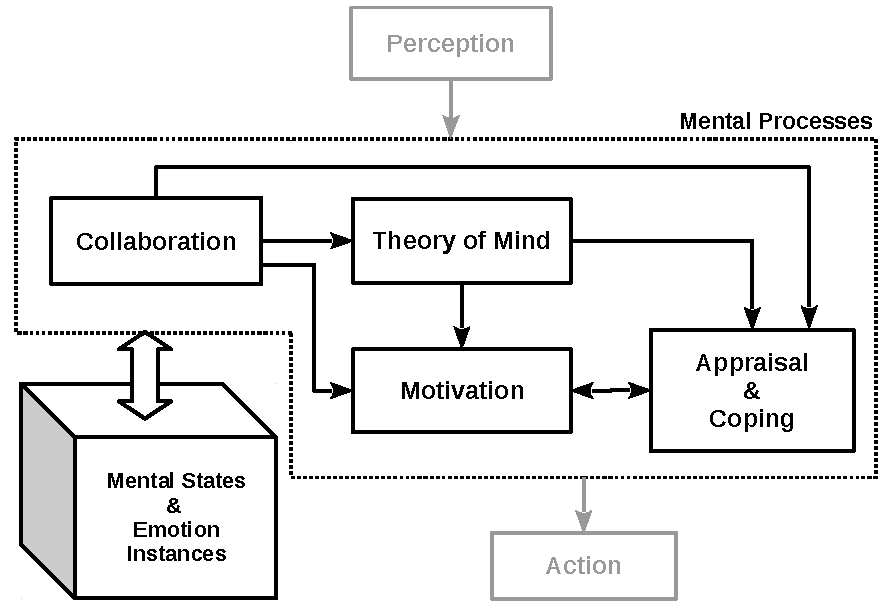
\includegraphics[width=0.474\textwidth]{figure/theory-general-croped.pdf}
  \caption{Computational framework based on Affective Motivational Collaboration
  Theory (arrows indicate primary influences between mechanisms).}
  \label{fig:cpm}
\end{figure}

\subsection{Mental States}

General description of mental states.

\subsubsection{Belief:}

Our description and the definition of attributes.

\subsubsection{Motive:}

Our description and the definition of attributes.

\subsubsection{Intention:}

Our description and the definition of attributes.

\subsubsection{Goal:}

Our description and the definition of attributes.

\subsubsection{Emotion Instance:}

Our description and one or two examples.

\subsection{Appraisal Process}

Short paragraph to describe appraisal process.

\section{Mental Graph}

A graph illustration of mental state and a clear short and desciptive
walkthrough example.

\begin{center}
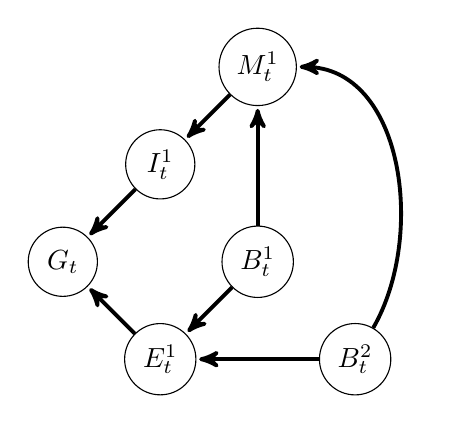
\begin{tikzpicture}[>=stealth',shorten >=1pt,node distance=1.75cm,on
grid,initial/.style    ={}] 
  \node[state]          (G)                         {$G_t$};
  \node[state]          (I1) [above right =of G]    {$I^1_t$};
  \node[state]          (E1) [below right =of G]    {$E^1_t$};
  \node[state]          (M1) [above right =of I1]   {$M^1_t$};
  \node[state]          (B1) [below right =of I1]   {$B^1_t$};
  \node[state]          (B2) [below right =of B1]   {$B^2_t$};
\tikzset{mystyle/.style={->,double=black}} 
\tikzset{every node/.style={fill=black}} 
\path (M1)    edge [mystyle]  (I1) 
      (B2)    edge [mystyle]  (E1)
      (I1)    edge [mystyle]  (G);
      (P)     edge [mystyle]  (M);
\tikzset{mystyle/.style={->,double=black}}   
\path (E1)    edge [mystyle]   (G)
      (B1)    edge [mystyle]   (E1) 
      (B1)    edge [mystyle]   (M1);
\tikzset{mystyle/.style={->,relative=false,in=0,out=60,double=black}}
\path (B2)    edge [mystyle]   (M1); 
\end{tikzpicture}
\end{center}

\section{Appraisal Processes}

A short paragraph to describe what variable we have chosen and why.

\subsection{Relevance}

Algorithm + Description + Example

\subsection{Desirability}

Algorithm + Description + Example

\subsection{Expectedness}

Algorithm + Description + Example

\subsection{Controllability}

Algorithm + Description + Example

\section{Conclusion}

Discussion about the application of the appraisal process in different
mechanisms in our computational theory including Motivation mechanism. 

\end{document}
